%(BEGIN_QUESTION)
% Copyright 2011, Tony R. Kuphaldt, released under the Creative Commons Attribution License (v 1.0)
% This means you may do almost anything with this work of mine, so long as you give me proper credit

Følgende P\&ID viser et FOUNDATION Fieldbus {\it kaskade}-reguleringssystem for regulering av væskenivå i en tank: en nivåregulator gir et «eksternt settpunkt»-signal til en strømningsregulator, som deretter regulerer hvor raskt væske strømmer ut av tanken:

$$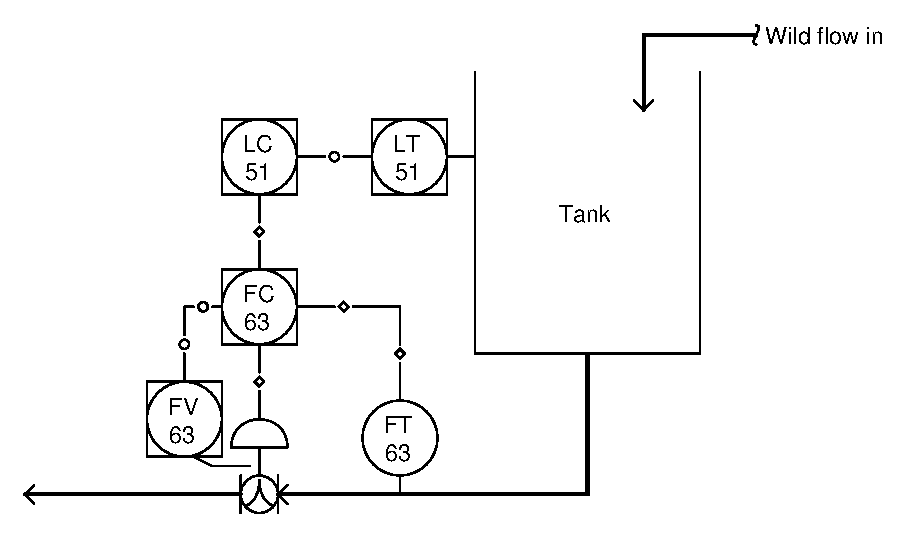
\includegraphics[width=15.5cm]{i00437x01.eps}$$

Et funksjonsblokkdiagram viser hvordan signalene er koblet sammen i dette Fieldbus-systemet:

$$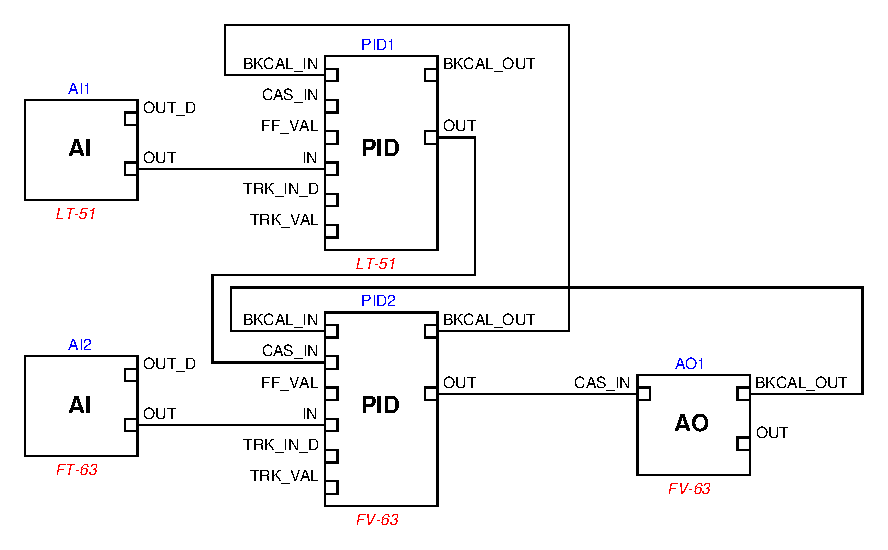
\includegraphics[width=15.5cm]{i00437x02.eps}$$

\filbreak

Basert på informasjonen som er gitt, avgjør hvilket av følgende {\it tidsdiagrammer} som passer denne Fieldbus-segmentkonfigurasjonen:

$$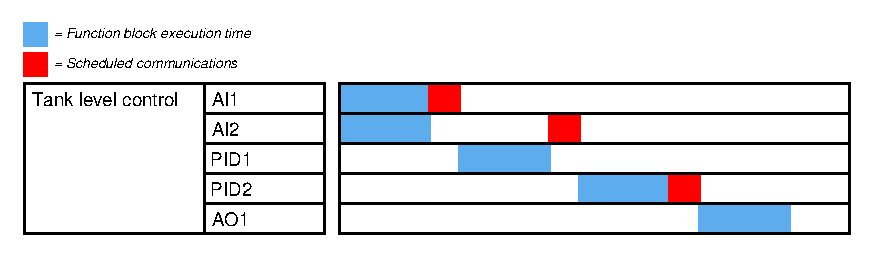
\includegraphics[width=15.5cm]{i00437x04.eps}$$

$$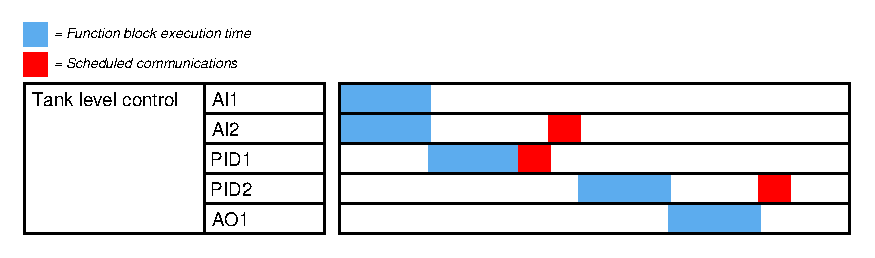
\includegraphics[width=15.5cm]{i00437x03.eps}$$  % This is the correct diagram!

$$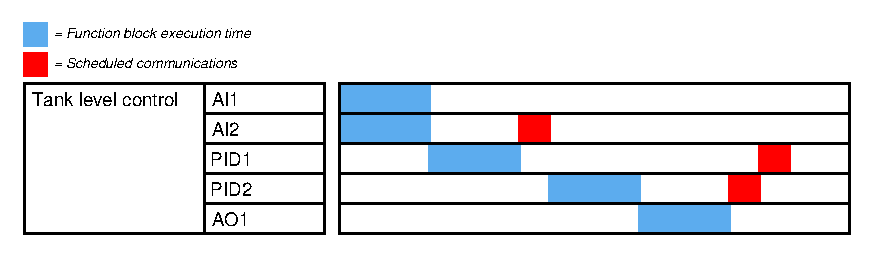
\includegraphics[width=15.5cm]{i00437x05.eps}$$ 

$$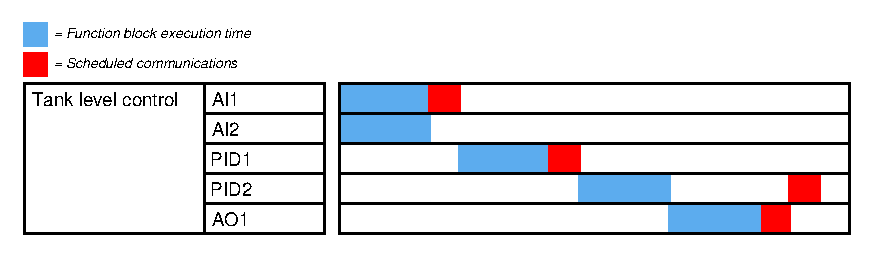
\includegraphics[width=15.5cm]{i00437x06.eps}$$ 

\underbar{file i00437}
%(END_QUESTION)





%(BEGIN_ANSWER)

$$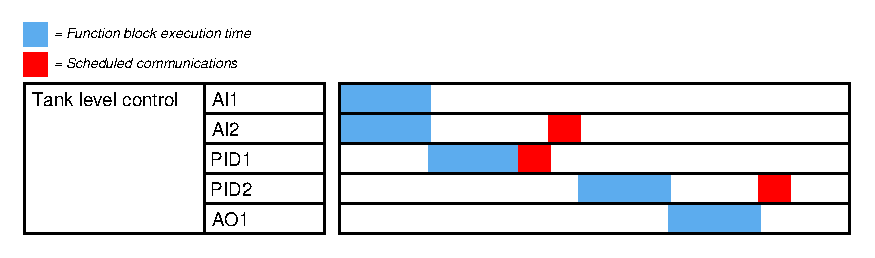
\includegraphics[width=15.5cm]{i00437x03.eps}$$  % This is the correct diagram!

%(END_ANSWER)





%(BEGIN_NOTES)

En nyttig problemløsningsstrategi er å bruke farger for å markere hvilke funksjonsblokker som ligger i samme feltinstrument:

$$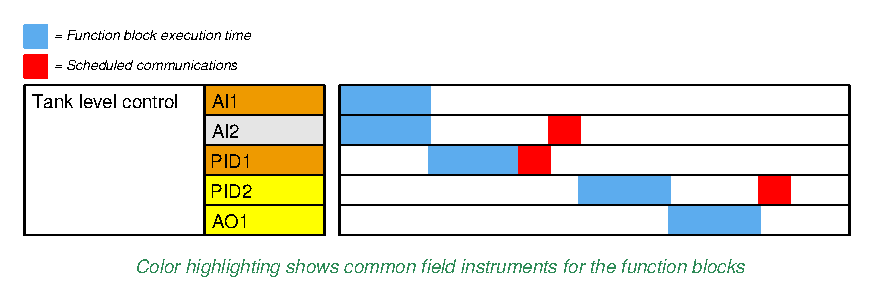
\includegraphics[width=15.5cm]{i00437x07.eps}$$  

En ledetråd for å identifisere riktig makrosyklusplan er å finne hvilke funksjonsblokker som må sende data ut på Fieldbus-nettverket, og hvilke blokker som ikke trenger å sende data på nettet i det hele tatt. Dette avhenger av blokkplassering (hvilket instrument blokken ligger i). Merk for eksempel at AI1 og PID1 begge ligger i samme enhet (LT-51), og derfor trenger ikke AI1 å sende utdata til PID1 på nettverket. Tilsvarende ligger PID2 og AO begge i ventilposisjoneren FV-63, og da trenger ikke PID2 å sende utdata til AO, og AO trenger heller ikke å sende BKCAL\_OUT-data til PID1.

\vskip 10pt

{\bf Blokker som trenger CD-token for å kringkaste data på Fieldbus-nettverket:}
\begin{itemize}
\item{} PID1
\item{} AI2
\item{} PID2
\end{itemize}

\vskip 10pt

{\bf Blokker som ikke trenger CD-token for å kringkaste data:}
\begin{itemize}
\item{} AI1
\item{} AO
\end{itemize}

Basert på disse listene kan ikke første og siste makrosyklus være riktige, fordi begge viser CD-token gitt til AI1- og AO-blokkene.

\vskip 10pt

Når vi ser på de to midterste tidsdiagrammene, spør vi hvilket som er mest fornuftig med tanke på rekkefølge. Av disse er \#2 mer fornuftig enn \#3, fordi \#3 lar PID1 sende utgangssignalet sitt som eksternt settpunkt til PID2 {\it etter} at PID2 allerede har sendt kommandosignal til ventilen. Det vil teknisk sett fungere, men krever to fulle makrosykluser for full informasjonsgjennomstrømming, mens planleggingen i \#2 bare krever én makrosyklus for å gjøre samme jobb.


%INDEX% Fieldbus, function block: block execution sequence
%INDEX% Fieldbus, function block: macrocycle

%(END_NOTES)
